\documentclass[letter, 10pt]{article}
\usepackage[utf8]{inputenc}
\usepackage[spanish]{babel}
\usepackage{amsfonts}
\usepackage{amsmath}
\usepackage{graphicx}
\usepackage{url}
\usepackage{algorithm}
\usepackage[noend]{algpseudocode}

\usepackage[top=3cm,bottom=3cm,left=3.5cm,right=3.5cm,footskip=1.5cm,headheight=1.5cm,headsep=.5cm,textheight=3cm]{geometry}

\def\BState{\State\hskip-\ALG@thistlm}

\begin{document}
\title{Inteligencia Artificial Avanzada \\ \begin{Large} Route selection for emergency logistics management\end{Large}}
\author{Maximiliano Osorio Bañados}
\date{\today}
\maketitle


\begin{abstract}
\textit{Route selection} es uno de los problemas fundamentales en la gestión de logística en caso de emergencia. En la literatura el problema ha sido tratado considerando la velocidad de viaje entre los nodos constante. Pero, la velocidad de viaje es variable con la extensión del desastre, especialmente en huracanes o inundaciones.
En este documento dos modelos matemáticos son presentados para la selección de rutas para emergencia: el primero, un modelo de un objetivo que considera el efecto del desastre en tiempo de viaje entre cada arco, o sea, el objetivo del modelo es minimizar el tiempo total de viaje a lo largo del camino y  el segundo, un modelo de multi objetivo donde busca minimizar el tiempo y el número de los nodos en el camino. Ambos resueltos con el uso de \textit{Ant colony system - TSP}
\end{abstract}

\section{Introducci\'on}
%Una explicaci\'on breve del contenido del informe. Es decir, detalla: Prop\'osito, Estructura del Documento, Descripci\'on (muy breve) del Problema y Motivaci\'on.

En los recientes años, los frecuentes desastres naturales y no naturales han producido una gran daño a la población, por ejemplo en Chile: Terremoto de 2010 en Concepción (27F), Gran Incendio de Valparaiso 2014 y Inundación del Norte de Chile en 2015, por lo cual es interesante observar los procedimientos de logística asociados a este tipo de desastres. La logística es una de las mayores actividades durante y después de la emergencia, la entrega de alimentos, medicamentos, abrigo deben ser entregados desde la zona de almacenamiento al área afectada de la manera más rápida posible. Es por eso que el diseño de rutas en casos de emergencia es un tema interesante de desarrollar. \\
En este documento se busca entender las variables que afectan al problema, su historia, consideraciones a tomar y los avances que se han realizado en la literatura. Para luego, en las próximas secciones describir de manera más amplia el problema, sus modelos y sus formas de resoluciones. Finalizando con las secciones relacionadas a la implementación donde se describirá la utilización de \textit{Ant Colony System} para el problema: representación utilizada, descripción del algoritmo diseñado, resultados y conclusiones. 

\section{Definici\'on del Problema}

%Explicaci\'on del problema que se va a estudiar, en que consiste, cuales son sus variables, restricciones y objetivos de manera general.
%Variantes m\'as conocidas que existen.
Definición de variables y parámetros:
\begin{itemize}
	\item Una red de emergencia es definida por un grafo directamente conectado $G(V,A)$, donde $V=\{v_1,v_2,\cdots, v_n\}$ es el conjunto de nodos y $A\subseteq V x V$ es el conjunto de arcos. Sea $V=\{v_1,v_2,\cdots, v_n\}$ los nodos en la red donde $v_1$ es el nodo inicial y $v_n$ es el nodo final.
	\item $i_{ij}$ denota el largo de los arcos que se encuentra entre los nodos $v_i$ y $v_j$, donde $(v_i,v_j) \in A$.
	\item $s_{ij}^0$ es la velocidad entre los arcos $(v_i,v_j)$ en condiciones normales. Sea $s_{ij}(t)$ es la velocidad de viaje en el arco $(v_i,v_j)$ bajos las condiciones del desastre en el tiempo t.\\

\begin{figure}[h]
\centering
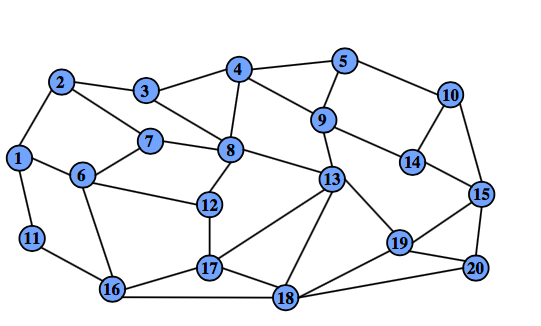
\includegraphics[scale=0.5]{images/routes.png}
\caption{Estructura de una red de emergencia}
\end{figure}
	
    A partir de la observación de desastre como huracanes y inundación. Se afirma que la velocidad de viaje en cada arco de la red decrece con el impacto del desastre. \cite{tufekci1995integrated} La disminución de la velocidad de viaje es dependiente a la posición del arco, el tipo de desastre, etc. Pero si perdida generalidad, la función de velocidad es dada por:
\begin{equation}
	  s_{ij}(t) = s_{ij}^0 \cdot \alpha_{ij} e^{-\beta_{ij}\cdot t}
\end{equation}
Donde \(\alpha_{ij}\) y \(\beta{ij}\) son los parámetros decrecientes que determinan la disminución de la velocidad del viaje \(s_{ij}(t)\), \(\alpha_{ij}\) y \(\beta{ij}\) pueden ser estimados a la distancia desde arco $(v_i,v_j)$ al centro del desastre, la vulnerabilidad del arco, el tipo de desastre, etc.
	\item Sea \(t_{ij}\) el tiempo necesario para viajar a través del arco $(v_i,v_j)$, se calcula como $t_{ij}=t_j-t_i$.
	\item Sea $x_i$ la ciudad visitada en la posición $i$
	\item P denota el camino que realizado, o sea es la secuencia de nodos en la redes que se elige. Sea $p_k$ el numero de la secuencia del nodo $v_{p_k}$	en la red, entonces P puede ser presentado como $(v_{p_1},v_{p_2},\cdots,v_{p_k}\cdots,v_{p_K})$ donde $1\leq p_k \leq n$ y k es la secuencia del nodo   $v_{p_k}$ en el camino P.  P debe iniciar en el nodo inicial $p_1=1$ y $p_K=n$. Y no deben existir ciclos.
	\item Sea $ET(P,v_{p_k})$ denota el tiempo de viaje desde el $v_{p_1}$ hasta $v_{p_k}$ a lo largo de $(v_{p_1},v_{p_2},\cdots,v_{p_k})$ donde $1\leq p_k \leq n$. A partir de eso se determina que:
	\begin{equation}
		ET(P,v_{p_k})= \sum_{m=1}^{k-1} t_{p_mp_{m+1}} = (t_{p_2} - t_{p_1}) +(t_{p_3} - t_{p_2}) + \cdots + (t_{p_k} - t_{p_{k-1}}) = t_{p_k}
	\end{equation}
	

\end{itemize}
 A partir de lo anterior podemos calcular el tiempo de un camino, dado que:
\begin{equation}\label{borde}
	  t_{p_1} = t_1 = 0
\end{equation} 
 
\begin{eqnarray}\label{int}
\int_{t_{p_{k-1}}}^{t_{p_k}} s_{p_{k-1}p_k}(t)dt = l_{p_{k-1}p_k} & & \text{\(2 \leq k \leq  K\)}\\
 \end{eqnarray}
 
En \eqref{int} conocemos el límite inferior de la integral, el integrando $ s_{p_{k-1}p_k}$ y el resultado de $ l_{p_{k-1}p_k} $ por lo tanto se puede obtener el limite superior $t_{p_k}$
Por recursividad se puede obtener los valores de $t_{p_k}$ para los nodos $v_{p_k}$ con  $1\leq p_k \leq n$.




\section{Estado del Arte}
%Lo m\'as importante que se ha hecho hasta ahora con relaci\'on al problema. Deber\'ia responder preguntas como las siguientes:
%?`cuando surge?, ?`qu\'e m\'etodos se han usado para resolverlo?, ?`cuales son los mejores algoritmos que se han creado hasta
%la fecha?, ?`qu\'e representaciones han tenido los mejores resultados?, ?`cu\'al es la tendencia actual?, tipos de movimientos,
%heur\'isticas, m\'etodos completos, tendencias, etc... Puede incluir gr\'aficos comparativos, o explicativos.\\

\textit{Path selection} es uno de los problemas fundamentales de logística. En los recientes años, los frecuentes desastres naturales ha incentivado la investigación en el área, pese a eso, las investigaciones en diseño de rutas para emergencias son acotadas.  Ozdamar et al. (2004) \cite{ozdamar2004emergency} construyeron un modelo para el diseño de rutas para emergencias, el objetivo es minimizar la demanda insatisfecha en la ruta planeada. El plan logístico de emergencia incluye los puntos óptimos de recoger y entregar los materiales en las rutas. Estas rutas son regeneradas mientras nuevos materiales y modos de transportes se vuelven disponibles durante el tiempo planeado, pero no considera que el tiempo de viaje en los nodos puede variar según el efecto de la catástrofe. Es  importante considerar este aspecto, según Farahmand (1997) \cite{farahmand1997application} y Tufekci  (1995) \cite{tufekci1995integrated} las condiciones de viaje entre los nodos se ven fuertemente afectadas por la extensión del desastre especialmente en desastre como huracanes e inundaciones que se extienden en tiempo y espacio, otros trabajos como Yuan and Wang (2009) \cite{Yuan20091081} construyeron un modelo para expresar el efecto de la extensión de un desastre para la velocidad de viaje, para la resolución de este problema utilizan dos técnicas: la primera basada en el algoritmo de Dijkstra, la idea es encontrar el camino más corto paso a paso y otro algoritmo que está basado en Ant colony optimization (ACO) \cite{Yuan20091081}. Xiaoge et al. (2013) \cite{zhang2013route} proponen un algoritmo inspirado en biología utilizando el comportamiento de las ameboides para calcular las rutas donde la velocidad los arcos en los nodos son variables. Investigaciones relacionadas han mostrado que las mayores congestiones cuando existe un desastre son producidas en las intersecciones de dos arcos en una ruta de emergencia Southworth (1991) \cite{southworth1991regional} y Cova (2003) \cite{cova2003network}, de hecho de ahí nace un nuevo problema \textit{Lane-based routing} donde la estrategia busca eliminar los cruces en las intersecciones con el fin de disminuir el tiempo en las intersecciones. \cite{cova2003network}


\section{Modelo Matem\'atico}
%Uno o m\'as modelos matem\'aticos para el problema, idealmente indicando elp espacio de b\'usqueda para cada uno.
Considerando lo descrito por Southworth (1991) \cite{southworth1991regional} y Cova (2003) \cite{cova2003network}: se diseñan dos modelos con distintos objetivos: el primero busca la minimización del tiempo y el segundo busca multiples objetivos: la minimización del tiempo y de la cantidad de nodos en la ruta.


\subsection{Minimización del tiempo} 

La formulación del \textit{path selection model} se describe de la siguiente manera:

El objetivo del modelo es minimizar el tiempo empleado en el camino. Las ecuaciones \eqref{7}, \eqref{8} y \eqref{9} son parte de la formula de recursión del tiempo total para el camino. En la ecuación \eqref{speed} la función decreciente de la velocidad de viaje en el arco $(v_i,v_j)$. La restricción \eqref{full} asegura un camino factible desde $v_1$ hasta $v_n$ y la restricción \eqref{circles} asegura que no existan ciclos.

\begin{equation}
	 \sum_{i=1}^{n}\sum_{j=1}^{n} t_{ij}x_{ij}
\end{equation}

\begin{equation}\label{7}
  \int_{t_i}^{t_j} s_{ij}(t)dt = l_{ij}
\end{equation}
\begin{equation}\label{8}
  t_{ij} = t_j - t_i
\end{equation}
\begin{equation}\label{9}
t_1 =0
\end{equation}
\begin{equation}\label{speed}
  s_{ij}(t) = s_{ij}^0 \cdot \alpha_{ij} e^{-\beta_{ij}\cdot t}
\end{equation}

\begin{equation}\label{full}
	\sum_{\substack{j=1\\
                  j \neq i}}^n x_{ij} - \sum_{\substack{j=1\\
                  j \neq i}}^{n} x_{ji} = \begin{cases}
1 & i=1\\
-1 & i=n \\
0 & eoc
\end{cases}
\end{equation}



\begin{equation}\label{circles}
	\sum_{\substack{j=1\\
                  j \neq i}}^n x_{ij} = \begin{cases}
\leq 1 & i\neq n\\
=0 & i=n 
\end{cases}
\end{equation}

\begin{equation}
	x_{ij} = 0,1;i=1,2,\cdots,n;j=1,2,\cdots,n
\end{equation}

\subsection{Multi-objetivo \textit{path selection}}

Southworth (1991) \cite{southworth1991regional} y Cova (2003) han mostrado que la mayor congestion sucede en las intersecciones de dos arcos en una red de emergencia, cuando se viaja en un camino con menor número de arcos es más fácil y rápido seguir el camino. La complejidad del camino puede obtenida por el número de arcos incluidos en un camino. 


\begin{equation}\label{f_1}
	min f_1 = \sum_{i=1}^{n}\sum_{j=1}^{n} t_{ij}x_{ij}
\end{equation}


\begin{equation}\label{f_2}
	min f_2 = \sum_{i=1}^{n}\sum_{j=1}^{n} x_{ij}
\end{equation}

La restricciones con la misma del modelo anterior.

\section{Descripción del algoritmo}

El algoritmo utilizado fue una implementación de Ant Colony System con TSP (ACS-TSP). Para la heurística se propuso en general:

\begin{equation}
	\eta_{ij} = r_1*\frac{f_1 - f_1^*}{f_1} + r_2*\frac{f_2 - f_2^*}{f_2}
\end{equation}

Donde $r_1$ y $r_2$ son los pesos asociados al tiempo y a la cantidad de nodos respectivamente, esto permite poder pasar del modelo multi-objetivo al modelo de minimización de tiempo fácilmente.  $f_1^m$ y $f_2^n$ son los valores de la función objetivo \eqref{f_1} y \eqref{f_2} que corresponde al camino encontrado por la hormiga $m$, $f_1^*$ y $f_2^*$ el mejor valor obtenido. Además $r_1$ y $r_2$ debe cumplir que $r_1 + r_2 = 1$

El algoritmo ACS-TSP modificado para el problema se describe:
\begin{itemize}
	\item Para cada arco $(i,j)$ se inicia $\tau_{ij}(0) = \tau_0$
	\item Para las $m$ hormigas, se posiciona cada una en el inicio.
	\item Iterar por cada hormiga hasta que se cumpla el tour de la siguiente manera:
	\begin{itemize}
	\item Se construye su camino se elige la siguiente ciudad, el movimiento esta definido por:
\begin{equation}
j = \begin{cases} arg max_{u \in S_{k}(i)} \{ [\tau(i,u)]^\alpha [\eta(i,u)]^\beta\} &\mbox{if } q \leq q_0 \\ 
J & otherwise \end{cases} 
\end{equation}

Donde $J \in J_i^k$ se elige según la probabilidad:

	\begin{equation}
		P_{ij}^k(t) = \frac{[\tau_{ij}(t)]^{\alpha_a}[\eta_{ij}]^{\beta_a}}{\sum_{h \in J_i^k } [\tau_{ij}(t)]^{\alpha_a}[\eta_{ij}]^{\beta_a}}
	\end{equation}
	
Y donde $i$ es la ciudad actual.
\item Luego se actualiza la feromona
\begin{equation}
	t_{ij}(t) = (1-\rho)t_{ij}(t) + \rho \tau_0
\end{equation}

	\end{itemize}

\item Salvar la mejor solución $T^+$, encontrada hasta el momento.
\item Para cada arco $(i,j) \in T^+$, se modifican los niveles de feromona aplicando:

\begin{equation}
	t_{ij}(t) = (1-\rho)t_{ij}(t) + \rho \Delta \tau_{ij}(t)
\end{equation}

donde $\Delta \tau_{ij}(t) = \frac{1}{L^+}$
\end{itemize} 
Los valores utilizados por $\alpha=1$,$\beta=2$,$q_0=0.9$,$m=10$,$Q=100$,$\tau_0=(nL_{nn})^{-1}$,$cl=15$
\section{Experimentos}

Basado en el trabajo de \cite{Yuan20091081} se busca estudiar el efecto de un mayor número de desastres y nivel de estos. A partir de la ecuación \eqref{speed}, se desprende que al disminuir $a_{ij}$ se refleja en la influencia instantánea de los desastres, un  $a_{ij}$ representa una gran influencia, $b_{ij}$ puede reflejarse en la influencia de los desastre en un periodo de tiempo donde el desastre sucede y un mayor $b_{ij}$ significa cuan rápido decrece la velocidad del viaje.


En el trabajo \cite{Yuan20091081} se observa, se dividió los 20 nodos en 3 áreas, que se muestra en la figura \ref{area3}. En cada área los parámetros decrecientes son generados en diferentes intervalos como se muestra en la figura. En cada área los parámetros son generados de forma aleatoria en los diferentes intervalos, los cuales se observan en el cuadro \ref{table:intervalo}. En el caso del desastre 0 es cuando nos encontramos en una situación sin ningún desastre y el desastre 5 es cuando nos encontramos en una situación más compleja.

\begin{figure}[H]
\centering
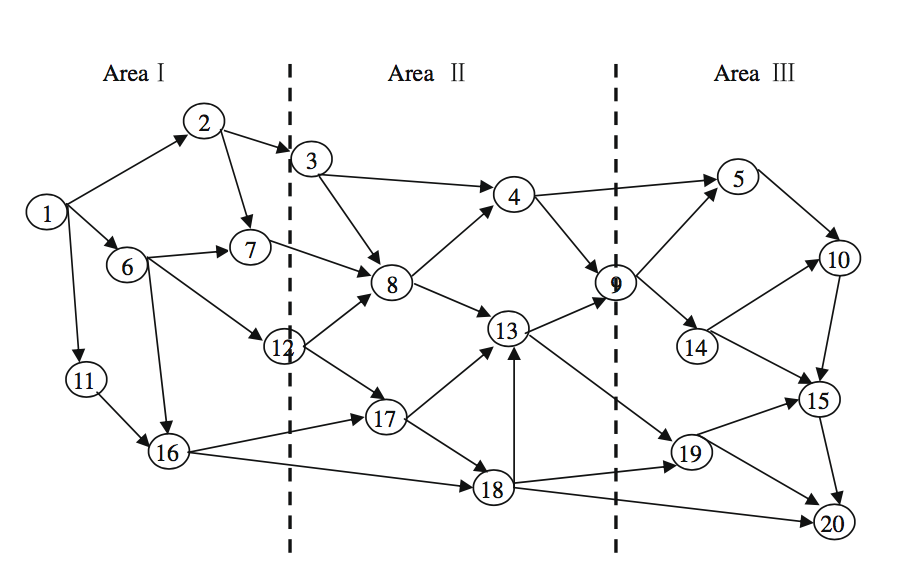
\includegraphics[scale=1]{images/areas.jpg}
\caption{División de una red de emergencia}\label{area3}

\end{figure}

En los cuadros \ref{grade1},\ref{grade2},\ref{grade3},\ref{grade4},\ref{grade5} se muestran los valores para los parametros $\alpha_{ij}$ y $\beta_{ij}$	de los distintos grados de desastre.



\begin{table}[H]
\centering
\begin{tabular}{|l|l|l|l|}
\hline
Tipo & Área I & Área II & Área III \\ \hline
Desastre 0 & $\alpha=1$,$\beta=0$ & $\alpha=1$,$\beta=0$ & $\alpha=1$,$\beta=0$ \\ \hline
Desastre 1 & $\alpha \in (0.9,1.0)$ $\beta \in (0.00,0.05)$ & $\alpha=1$,$\beta=0$ & $\alpha=1$,$\beta=0$ \\ \hline
Desastre 2 & $\alpha \in (0.8,0.9)$ $\beta \in (0.05,0.10)$ & $\alpha \in (0.9,1.0)$ $\beta \in (0.00,0.05)$ & $\alpha=1$,$\beta=0$ \\ \hline
Desastre 3 & $\alpha \in (0.7,0.8)$ $\beta \in (0.10,0.15)$ & $\alpha \in (0.8,0.9)$ $\beta \in (0.05,0.10)$ & $\alpha \in (0.9,1.0)$ $\beta \in (0.00,0.05)$ \\ \hline
Desastre 4 & $\alpha \in (0.6,0.7)$ $\beta \in (0.15,0.20)$ & $\alpha \in (0.7,0.8)$ $\beta \in (0.10,0.15)$ & $\alpha \in (0.8,0.9)$ $\beta \in (0.05,0.10)$ \\ \hline
Desastre 5 & $\alpha \in (0.5,0.6)$ $\beta \in (0.20,0.25)$ & $\alpha \in (0.6,0.7)$ $\beta \in (0.15,0.20)$ &  $\alpha \in (0.7,0.8)$  $\beta \in (0.10,0.15)$\\ \hline
\end{tabular}
\caption{Intervalos de los parametros por área}\label{table:intervalo}
\end{table}




\begin{table}[H]
\centering
\begin{tabular}{|l|l|l|l|l|l|}
\hline
inicio & fin & $l_{i,j}$ & $s_{i,j}$ & $\alpha_{i,j}$ & $\beta_{i,j}$ \\ \hline
1 & 2 & 50 & 100 & 0.9222 & 0.0381 \\ \hline
1 & 6 & 30 & 60 & 0.9193 & 0.0143 \\ \hline
1 & 11 & 70 & 110 & 0.9022 & 0.0499 \\ \hline
2 & 3 & 30 & 60 & 0.9904 & 0.0277 \\ \hline
2 & 7 & 40 & 70 & 0.9857 & 0.0305 \\ \hline
6 & 7 & 30 & 65 & 0.9577 & 0.0123 \\ \hline
6 & 12 & 60 & 105 & 0.906 & 0.0399 \\ \hline
6 & 16 & 100 & 115 & 0.9049 & 0.0353 \\ \hline
7 & 8 & 40 & 90 & 0.9153 & 0.0436 \\ \hline
11 & 16 & 30 & 70 & 0.9967 & 0.0089 \\ \hline
16 & 17 & 80 & 115 & 0.964 & 0.0491 \\ \hline
16 & 18 & 110 & 120 & 0.9294 & 0.0327 \\ \hline
3 & 4 & 80 & 100 & 1 & 0 \\ \hline
3 & 8 & 60 & 95 & 1 & 0 \\ \hline
4 & 5 & 110 & 120 & 1 & 0 \\ \hline
4 & 9 & 40 & 75 & 1 & 0 \\ \hline
5 & 10 & 60 & 110 & 1 & 0 \\ \hline
8 & 4 & 40 & 85 & 1 & 0 \\ \hline
8 & 13 & 30 & 75 & 1 & 0 \\ \hline
9 & 5 & 70 & 110 & 1 & 0 \\ \hline
9 & 14 & 40 & 90 & 1 & 0 \\ \hline
10 & 15 & 50 & 105 & 1 & 0 \\ \hline
12 & 8 & 30 & 65 & 1 & 0 \\ \hline
12 & 17 & 40 & 100 & 1 & 0 \\ \hline
13 & 9 & 30 & 80 & 1 & 0 \\ \hline
13 & 19 & 110 & 120 & 1 & 0 \\ \hline
14 & 10 & 80 & 115 & 1 & 0 \\ \hline
14 & 15 & 60 & 105 & 1 & 0 \\ \hline
15 & 20 & 30 & 90 & 1 & 0 \\ \hline
17 & 13 & 40 & 80 & 1 & 0 \\ \hline
17 & 18 & 40 & 75 & 1 & 0 \\ \hline
18 & 13 & 60 & 115 & 1 & 0 \\ \hline
18 & 19 & 70 & 110 & 1 & 0 \\ \hline
18 & 20 & 120 & 120 & 1 & 0 \\ \hline
19 & 15 & 40 & 75 & 1 & 0 \\ \hline
19 & 20 & 70 & 105 & 1 & 0 \\ \hline

\end{tabular}
\caption{Parámetros para un desastre grado 1}
\label{grade1}
\end{table}


\begin{table}[H]
\centering
\begin{tabular}{|l|l|l|l|l|l|}
\hline
inicio & fin & $l_{i,j}$ & $s_{i,j}$ & $\alpha_{i,j}$ & $\beta_{i,j}$ \\ \hline
1 & 2 & 50 & 100 & 0.9222 & 0.0381 \\ \hline
1 & 6 & 30 & 60 & 0.9193 & 0.0143 \\ \hline
1 & 11 & 70 & 110 & 0.9022 & 0.0499 \\ \hline
2 & 3 & 30 & 60 & 0.9904 & 0.0277 \\ \hline
2 & 7 & 40 & 70 & 0.9857 & 0.0305 \\ \hline
6 & 7 & 30 & 65 & 0.9577 & 0.0123 \\ \hline
6 & 12 & 60 & 105 & 0.906 & 0.0399 \\ \hline
6 & 16 & 100 & 115 & 0.9049 & 0.0353 \\ \hline
7 & 8 & 40 & 90 & 0.9153 & 0.0436 \\ \hline
11 & 16 & 30 & 70 & 0.9967 & 0.0089 \\ \hline
16 & 17 & 80 & 115 & 0.964 & 0.0491 \\ \hline
16 & 18 & 110 & 120 & 0.9294 & 0.0327 \\ \hline
3 & 4 & 80 & 100 & 0.9153 & 0.0216 \\ \hline
3 & 8 & 60 & 95 & 0.9562 & 0.0114 \\ \hline
4 & 5 & 110 & 120 & 0.989 & 0.0281 \\ \hline
4 & 9 & 40 & 75 & 0.9984 & 0.0386 \\ \hline
8 & 4 & 40 & 85 & 0.9746 & 0.0376 \\ \hline
8 & 13 & 30 & 75 & 0.9999 & 0.0222 \\ \hline
12 & 8 & 30 & 65 & 0.9345 & 0.0044 \\ \hline
12 & 17 & 40 & 100 & 0.9846 & 0.0228 \\ \hline
13 & 9 & 30 & 80 & 0.9094 & 0.0264 \\ \hline
13 & 19 & 110 & 120 & 0.9326 & 0.0151 \\ \hline
17 & 13 & 40 & 80 & 0.9077 & 0.035 \\ \hline
17 & 18 & 40 & 75 & 0.947 & 0.0344 \\ \hline
18 & 13 & 60 & 115 & 0.9669 & 0.0202 \\ \hline
18 & 19 & 70 & 110 & 0.953 & 0.0059 \\ \hline
18 & 20 & 120 & 120 & 0.9278 & 0.0021 \\ \hline
5 & 10 & 60 & 110 & 1 & 0 \\ \hline
9 & 5 & 70 & 110 & 1 & 0 \\ \hline
9 & 14 & 40 & 90 & 1 & 0 \\ \hline
10 & 15 & 50 & 105 & 1 & 0 \\ \hline
14 & 10 & 80 & 115 & 1 & 0 \\ \hline
14 & 15 & 60 & 105 & 1 & 0 \\ \hline
15 & 20 & 30 & 90 & 1 & 0 \\ \hline
19 & 15 & 40 & 75 & 1 & 0 \\ \hline
19 & 20 & 70 & 105 & 1 & 0 \\ \hline
\end{tabular}
\caption{Parámetros para un desastre grado 2}
\label{grade2}
\end{table}

\begin{table}[H]
\centering
\begin{tabular}{|l|l|l|l|l|l|}
\hline
inicio & fin & $l_{i,j}$ & $s_{i,j}$ & $\alpha_{i,j}$ & $\beta_{i,j}$ \\ \hline
1 & 2 & 50 & 100 & 0.7544 & 0.1026 \\ \hline
1 & 6 & 30 & 60 & 0.7666 & 0.1394 \\ \hline
1 & 11 & 70 & 110 & 0.7561 & 0.1276 \\ \hline
2 & 3 & 30 & 60 & 0.7071 & 0.1089 \\ \hline
2 & 7 & 40 & 70 & 0.7527 & 0.1277 \\ \hline
6 & 7 & 30 & 65 & 0.7001 & 0.1062 \\ \hline
6 & 12 & 60 & 105 & 0.7145 & 0.1209 \\ \hline
6 & 16 & 100 & 115 & 0.7234 & 0.1361 \\ \hline
7 & 8 & 40 & 90 & 0.7242 & 0.108 \\ \hline
11 & 16 & 30 & 70 & 0.7378 & 0.1281 \\ \hline
16 & 17 & 80 & 115 & 0.7048 & 0.1197 \\ \hline
16 & 18 & 110 & 120 & 0.7639 & 0.1365 \\ \hline
3 & 4 & 80 & 100 & 0.8912 & 0.0844 \\ \hline
3 & 8 & 60 & 95 & 0.8242 & 0.0571 \\ \hline
4 & 5 & 110 & 120 & 0.8773 & 0.0552 \\ \hline
4 & 9 & 40 & 75 & 0.8678 & 0.099 \\ \hline
8 & 4 & 40 & 85 & 0.8801 & 0.067 \\ \hline
8 & 13 & 30 & 75 & 0.8425 & 0.0987 \\ \hline
12 & 8 & 30 & 65 & 0.8383 & 0.0543 \\ \hline
12 & 17 & 40 & 100 & 0.8785 & 0.0786 \\ \hline
13 & 9 & 30 & 80 & 0.8551 & 0.0707 \\ \hline
13 & 19 & 110 & 120 & 0.873 & 0.057 \\ \hline
17 & 13 & 40 & 80 & 0.8191 & 0.0778 \\ \hline
17 & 18 & 40 & 75 & 0.8555 & 0.0781 \\ \hline
18 & 13 & 60 & 115 & 0.8965 & 0.0653 \\ \hline
18 & 19 & 70 & 110 & 0.8967 & 0.0694 \\ \hline
18 & 20 & 120 & 120 & 0.8551 & 0.0948 \\ \hline
5 & 10 & 60 & 110 & 0.9476 & 0.0343 \\ \hline
9 & 5 & 70 & 110 & 0.9806 & 0.0484 \\ \hline
9 & 14 & 40 & 90 & 0.9984 & 0.0219 \\ \hline
10 & 15 & 50 & 105 & 0.9937 & 0.0091 \\ \hline
14 & 10 & 80 & 115 & 0.9334 & 0.0486 \\ \hline
14 & 15 & 60 & 105 & 0.9966 & 0.022 \\ \hline
15 & 20 & 30 & 90 & 0.9517 & 0.0363 \\ \hline
19 & 15 & 40 & 75 & 0.9547 & 0.0265 \\ \hline
19 & 20 & 70 & 105 & 0.9849 & 0.029 \\ \hline
\end{tabular}
\caption{Parámetros para un desastre grado 3}\label{grade3}
\end{table}


\begin{table}[H]
\centering
\begin{tabular}{|l|l|l|l|l|l|}
\hline
inicio & fin & $l_{i,j}$ & $s_{i,j}$ & $\alpha_{i,j}$ & $\beta_{i,j}$ \\ \hline
1 & 2 & 50 & 100 & 0.6396 & 0.1783 \\ \hline
1 & 6 & 30 & 60 & 0.6815 & 0.1934 \\ \hline
1 & 11 & 70 & 110 & 0.6204 & 0.1647 \\ \hline
2 & 3 & 30 & 60 & 0.6244 & 0.1698 \\ \hline
2 & 7 & 40 & 70 & 0.658 & 0.1674 \\ \hline
6 & 7 & 30 & 65 & 0.6481 & 0.1515 \\ \hline
6 & 12 & 60 & 105 & 0.6717 & 0.1957 \\ \hline
6 & 16 & 100 & 115 & 0.6706 & 0.1672 \\ \hline
7 & 8 & 40 & 90 & 0.6619 & 0.1864 \\ \hline
11 & 16 & 30 & 70 & 0.6821 & 0.1645 \\ \hline
16 & 17 & 80 & 115 & 0.6146 & 0.1858 \\ \hline
16 & 18 & 110 & 120 & 0.6625 & 0.1918 \\ \hline
3 & 4 & 80 & 100 & 0.7606 & 0.1184 \\ \hline
3 & 8 & 60 & 95 & 0.7454 & 0.1348 \\ \hline
4 & 5 & 110 & 120 & 0.7276 & 0.1178 \\ \hline
4 & 9 & 40 & 75 & 0.7686 & 0.1192 \\ \hline
8 & 4 & 40 & 85 & 0.7416 & 0.1484 \\ \hline
8 & 13 & 30 & 75 & 0.7073 & 0.132 \\ \hline
12 & 8 & 30 & 65 & 0.7911 & 0.1081 \\ \hline
12 & 17 & 40 & 100 & 0.7222 & 0.117 \\ \hline
13 & 9 & 30 & 80 & 0.7869 & 0.1274 \\ \hline
13 & 19 & 110 & 120 & 0.7775 & 0.1477 \\ \hline
17 & 13 & 40 & 80 & 0.7769 & 0.1329 \\ \hline
17 & 18 & 40 & 75 & 0.7269 & 0.1441 \\ \hline
18 & 13 & 60 & 115 & 0.711 & 0.1483 \\ \hline
18 & 19 & 70 & 110 & 0.7779 & 0.1018 \\ \hline
18 & 20 & 120 & 120 & 0.7046 & 0.127 \\ \hline
5 & 10 & 60 & 110 & 0.8334 & 0.0652 \\ \hline
9 & 5 & 70 & 110 & 0.8208 & 0.0519 \\ \hline
9 & 14 & 40 & 90 & 0.8827 & 0.0574 \\ \hline
10 & 15 & 50 & 105 & 0.8225 & 0.0678 \\ \hline
14 & 10 & 80 & 115 & 0.8736 & 0.0859 \\ \hline
14 & 15 & 60 & 105 & 0.8742 & 0.0662 \\ \hline
15 & 20 & 30 & 90 & 0.8935 & 0.0502 \\ \hline
19 & 15 & 40 & 75 & 0.8001 & 0.0811 \\ \hline
19 & 20 & 70 & 105 & 0.8535 & 0.0919 \\ \hline
\end{tabular}
\caption{Parámetros para un desastre grado 4}\label{grade4}
\end{table}


\begin{table}[H]
\centering
\begin{tabular}{|l|l|l|l|l|l|}
\hline
inicio & fin & $l_{i,j}$ & $s_{i,j}$ & $\alpha_{i,j}$ & $\beta_{i,j}$ \\ \hline
1 & 2 & 50 & 100 & 0.5335 & 0.2015 \\ \hline
1 & 6 & 30 & 60 & 0.5102 & 0.2404 \\ \hline
1 & 11 & 70 & 110 & 0.5288 & 0.2376 \\ \hline
2 & 3 & 30 & 60 & 0.5413 & 0.2201 \\ \hline
2 & 7 & 40 & 70 & 0.5049 & 0.2283 \\ \hline
6 & 7 & 30 & 65 & 0.5423 & 0.2267 \\ \hline
6 & 12 & 60 & 105 & 0.5016 & 0.2193 \\ \hline
6 & 16 & 100 & 115 & 0.5914 & 0.2336 \\ \hline
7 & 8 & 40 & 90 & 0.5212 & 0.2217 \\ \hline
11 & 16 & 30 & 70 & 0.5772 & 0.2161 \\ \hline
16 & 17 & 80 & 115 & 0.5936 & 0.2269 \\ \hline
16 & 18 & 110 & 120 & 0.5795 & 0.2271 \\ \hline
3 & 4 & 80 & 100 & 0.6196 & 0.156 \\ \hline
3 & 8 & 60 & 95 & 0.6887 & 0.1668 \\ \hline
4 & 5 & 110 & 120 & 0.64 & 0.1504 \\ \hline
4 & 9 & 40 & 75 & 0.6957 & 0.1961 \\ \hline
8 & 4 & 40 & 85 & 0.6951 & 0.1611 \\ \hline
8 & 13 & 30 & 75 & 0.6613 & 0.1619 \\ \hline
12 & 8 & 30 & 65 & 0.6174 & 0.1741 \\ \hline
12 & 17 & 40 & 100 & 0.6164 & 0.1711 \\ \hline
13 & 9 & 30 & 80 & 0.6271 & 0.1899 \\ \hline
13 & 19 & 110 & 120 & 0.6139 & 0.1851 \\ \hline
17 & 13 & 40 & 80 & 0.6382 & 0.1995 \\ \hline
17 & 18 & 40 & 75 & 0.6247 & 0.1973 \\ \hline
18 & 13 & 60 & 115 & 0.6339 & 0.1579 \\ \hline
18 & 19 & 70 & 110 & 0.6754 & 0.1805 \\ \hline
18 & 20 & 120 & 120 & 0.6687 & 0.1729 \\ \hline
5 & 10 & 60 & 110 & 0.7393 & 0.1177 \\ \hline
9 & 5 & 70 & 110 & 0.7387 & 0.1479 \\ \hline
9 & 14 & 40 & 90 & 0.7823 & 0.1425 \\ \hline
10 & 15 & 50 & 105 & 0.7584 & 0.13 \\ \hline
14 & 10 & 80 & 115 & 0.7348 & 0.1106 \\ \hline
14 & 15 & 60 & 105 & 0.7513 & 0.1019 \\ \hline
15 & 20 & 30 & 90 & 0.7585 & 0.1131 \\ \hline
19 & 15 & 40 & 75 & 0.7808 & 0.1341 \\ \hline
19 & 20 & 70 & 105 & 0.7903 & 0.104 \\ \hline
\end{tabular}
\caption{Parámetros para un desastre grado 5}\label{grade5}
\end{table}

Otro experimento realizado fue observar la sensibilidad de los resultados de tiempo y largo respecto a cambio de $r_1$ y $r_2$ en el intervalo $[0.05,0.95]$ con un salto de $0.05$ con el fin de estudiar si existe dependencia de $r_1$ y $r_2$ con el problema o las instancias a resolver.
\section{Resultados}

Para comparar los resultados obtenidos por el algoritmo (ACS-TSP) se usarán los resultados obtenidos por Yuan (2009) \cite{Yuan20091081} donde utiliza un algoritmo de \textit{Best path Dijkstra} y otro de \textit{Static shortest path}. \\

Como se muestra en los cuadros \ref{res-grade-1},\ref{res-grade-2},\ref{res-grade-3},\ref{res-grade-4},\ref{res-grade-5} ACS-TSP obtiene los mejores valores del problema al igual que \textit{Best path Dijkstra} y mejores que \textit{Static shortest path} ambos propuestos por  Yuan (2009)\cite{Yuan20091081}
\begin{table}[H]
\centering
\begin{tabular}{|l|l|l|}
\hline
Algoritmo            & Camino           & Tiempo {[}min{]} \\ \hline
Best path Dijkstra   & 1 $\rightarrow$ 6$\rightarrow$12$\rightarrow$17$\rightarrow$18$\rightarrow$20 & 3.136548         \\ \hline
Static shortest path & 1$\rightarrow$11$\rightarrow$16$\rightarrow$18$\rightarrow$20    & 3.196073         \\ \hline
ACS-TSP              & 1$\rightarrow$6$\rightarrow$12$\rightarrow$17$\rightarrow$18$\rightarrow$20 & 3.136548         \\ \hline
\end{tabular}
\caption{Resultado grado 1}
\label{res-grade-1}
\end{table}

\begin{table}[H]
\centering
\begin{tabular}{|l|l|l|}
\hline
Algoritmo            & Camino           & Tiempo {[}min{]} \\ \hline
Best path Dijkstra   & 1 $\rightarrow$ 6$\rightarrow$12$\rightarrow$17$\rightarrow$18$\rightarrow$20 & 3.480311         \\ \hline
Static shortest path & 1$\rightarrow$11$\rightarrow$16$\rightarrow$18$\rightarrow$20    & 3.694391         \\ \hline
ACS-TSP              & 1$\rightarrow$6$\rightarrow$12$\rightarrow$17$\rightarrow$18$\rightarrow$20 & 3.480311         \\ \hline
\end{tabular}
\caption{Resultado grado 2}
\label{res-grade-2}
\end{table}

\begin{table}[H]
\centering
\begin{tabular}{|l|l|l|}
\hline
Algoritmo            & Camino           & Tiempo {[}min{]} \\ \hline
Best path Dijkstra   & 1 $\rightarrow$ 6$\rightarrow$12$\rightarrow$17$\rightarrow$18$\rightarrow$20 & 4.544814         \\ \hline
Static shortest path & 1$\rightarrow$11$\rightarrow$16$\rightarrow$18$\rightarrow$20    & 4.954273         \\ \hline
ACS-TSP              & 1$\rightarrow$6$\rightarrow$12$\rightarrow$17$\rightarrow$18$\rightarrow$20 & 4.544814         \\ \hline
\end{tabular}
\caption{Resultado grado 3}
\label{res-grade-3}
\end{table}


\begin{table}[H]
\centering
\begin{tabular}{|l|l|l|}
\hline
Algoritmo            & Camino           & Tiempo {[}min{]} \\ \hline
Best path Dijkstra   & 1 $\rightarrow$ 6$\rightarrow$12$\rightarrow$8$\rightarrow$13$\rightarrow$9$\rightarrow$14$\rightarrow$15$\rightarrow$20& 6.365086         \\ \hline
Static shortest path & 1$\rightarrow$11$\rightarrow$16$\rightarrow$18$\rightarrow$20    & 7.468316         \\ \hline
ACS-TSP              & 1 $\rightarrow$ 6$\rightarrow$12$\rightarrow$8$\rightarrow$13$\rightarrow$9$\rightarrow$14$\rightarrow$15$\rightarrow$20& 6.365086        \\ \hline
\end{tabular}
\caption{Resultado grado 4}
\label{res-grade-4}
\end{table}


\begin{table}[H]
\centering
\begin{tabular}{|l|l|l|}
\hline
Algoritmo            & Camino           & Tiempo {[}min{]} \\ \hline
Best path Dijkstra   & 1 $\rightarrow$ 2$\rightarrow$3$\rightarrow$4$\rightarrow$9$\rightarrow$14$\rightarrow$15$\rightarrow$20 & 12.323639         \\ \hline
Static shortest path & 1$\rightarrow$11$\rightarrow$16$\rightarrow$18$\rightarrow$20    & 19.297973         \\ \hline
ACS-TSP              & 1 $\rightarrow$ 2$\rightarrow$3$\rightarrow$4$\rightarrow$9$\rightarrow$14$\rightarrow$15$\rightarrow$20 & 12.323639         \\ \hline
\end{tabular}
\caption{Resultado grado 5}
\label{res-grade-5}
\end{table}

Al estudiar la sensibilidad de los resultados cambiando el valor de $r_1$ tal que $r_1 + r_2 = 1$ se puede observar en las instancias propuestas, los caminos con mayor número de nodos tienen un menor tiempo asociados, esto es producido debido a que al entregar un mayor peso a la minimización de cantidad de nodos en la ruta se eligen rutas con alto tiempo para poder realizar la minimización.
\begin{table}[H]
\centering
\begin{tabular}{|l|l|l|l|}
\hline
$r_1$ & min & tiempo {[}min{]} & largo \\ \hline
0.05 & 0.238405  & 3.19333 & 5 \\ \hline
0.1  & 0.22681   & 3.19333 & 5 \\ \hline
0.15 & 0.215216  & 3.19333 & 5 \\ \hline
0.2  & 0.203621  & 3.19333 & 5 \\ \hline
0.25 & 0.192026  & 3.19333 & 5 \\\hline
0.3  & 0.180431  & 3.19333 & 5 \\\hline
0.35 & 0.168837  & 3.19333 & 5 \\\hline
0.4  & 0.157242  & 3.19333 & 5 \\\hline
0.45 & 0.145647  & 3.19333 & 5 \\\hline
0.5  & 0.134052  & 3.19333 & 5 \\\hline
0.55 & 0.122458  & 3.19333 & 5 \\\hline
0.6  & 0.110863  & 3.19333 & 5 \\\hline
0.65 & 0.0992681 & 3.19333 & 5 \\\hline
0.7  & 0.0876734 & 3.19333 & 5 \\\hline
0.75 & 0.0760786 & 3.19333 & 5 \\\hline
0.8  & 0.0644838 & 3.19333 & 5 \\\hline
0.85 & 0.0528891 & 3.19333 & 5 \\\hline
0.9  & 0.0412943 & 3.19333 & 5 \\\hline
0.95 & 0.0237405 & 3.13239 & 6 \\\hline
\end{tabular}
\caption{Análisis de sensibilidad para grado 1}
\label{ses-1}
\end{table}



\begin{table}[H]
\centering
\begin{tabular}{|l|l|l|l|}
\hline
$r_1$ & min & tiempo {[}min{]} & largo \\ \hline
0.05 & 0.246164 & 7.46814 & 5 \\ \hline
0.1 & 0.242329 & 7.46814 & 5 \\ \hline
0.15 & 0.238493 & 7.46814 & 5 \\ \hline
0.2 & 0.234658 & 7.46814 & 5 \\ \hline
0.25 & 0.230822 & 7.46814 & 5 \\ \hline
0.3 & 0.226987 & 7.46814 & 5 \\ \hline
0.35 & 0.223151 & 7.46814 & 5 \\ \hline
0.4 & 0.219316 & 7.46814 & 5 \\ \hline
0.45 & 0.21548 & 7.46814 & 5 \\ \hline
0.5 & 0.211644 & 7.46814 & 5 \\ \hline
0.55 & 0.207809 & 7.46814 & 5 \\ \hline
0.6 & 0.203973 & 7.46814 & 5 \\ \hline
0.65 & 0.187646 & 6.48896 & 6 \\ \hline
0.7 & 0.163618 & 6.48896 & 6 \\ \hline
0.75 & 0.139591 & 6.48896 & 6 \\ \hline
0.8 & 0.115564 & 6.48896 & 6 \\ \hline
0.85 & 0.0915365 & 6.48896 & 6 \\ \hline
0.9 & 0.0675092 & 6.48896 & 6 \\ \hline
\end{tabular}
\caption{Análisis de sensibilidad para grado 4}
\label{ses-4}
\end{table}


\begin{table}[H]
\centering
\begin{tabular}{|l|l|l|l|}
\hline
$r_1$ & min & tiempo {[}min{]} & largo \\ \hline
0.05 & 0.265712  & 19.2772 & 5 \\ \hline
0.1  & 0.281425  & 19.2772 & 5 \\ \hline
0.15 & 0.297137  & 19.2772 & 5 \\ \hline
0.2  & 0.312849  & 19.2772 & 5 \\ \hline
0.25 & 0.328562  & 19.2772 & 5 \\ \hline
0.3  & 0.344274  & 19.2772 & 5 \\ \hline
0.35 & 0.359986  & 19.2772 & 5 \\ \hline
0.4  & 0.375699  & 19.2772 & 5 \\ \hline
0.45 & 0.382653  & 15.2718 & 6 \\ \hline
0.5  & 0.369615  & 15.2718 & 6 \\ \hline
0.55 & 0.356576  & 15.2718 & 6 \\ \hline
0.6  & 0.375501  & 15.9283 & 6 \\ \hline
0.65 & 0.365126  & 15.9283 & 6 \\ \hline
0.7  & 0.354752  & 15.9283 & 6 \\ \hline
0.75 & 0.250165  & 12.3264 & 8 \\ \hline
0.8  & 0.200176  & 12.3264 & 8 \\ \hline
0.85 & 0.15622   & 12.3264 & 8 \\ \hline
0.9  & 0.100198  & 12.3264 & 8 \\ \hline
0.95 & 0.0502092 & 12.3264 & 8 \\ \hline
\end{tabular}
\caption{Análisis de sensibilidad para grado 5}
\label{ses-5}
\end{table}

Respecto a los tiempos de uso de computacional del algoritmo, en el cuadro \ref{time} se muestra los tiempos asociados a cada grado de desastre en segundos, se puede afirmar que los tiempos que se encuentran entre $[8, 44]$ ms.

\begin{table}[H]
\centering
\begin{tabular}{|l|l|l|l|l|}
\hline
Grado 1 [s] & Grado 2 [s] & Grado 3  [s] & Grado 4 [s]& Grado 5 [s]\\ \hline
$0.00784\pm0.0049$ & $0.01702\pm0.0069$ & $0.025236\pm0.0048$ & $0.03304\pm0.0046$ & $0.04304\pm0.0462$ \\ \hline\end{tabular}
\caption{Tiempos del peor caso}
\label{time}
\end{table}

\section{Conclusiones}


El modelo I únicamente considera el efecto del desastre sobre el tiempo y la velocidad de viaje en cada arco, por lo tanto nos entrega un resultado independiente a parámetros, en cambio el modelo II al considerar multiples objetivos quedará dependiente del parámetro del peso. Pero como puede se puede observar en el documento es sumamente importante de considerar el objetivo de la minimización de los nodos dado que afecta directamente al objetivo del tiempo.

%El diseño de la heurística para la situación es de suma importancia para obtener un función objetivo fiable. En el problema debe comparar el peso de la minimización de la cantidad de nodos en la ruta y el peso de la minimización del tiempo. 

Para partir de los resultados,  \textit{Ant Colony System - TSP} es una técnica muy adecuada para este tipo de problema, ya que el problema de \textit{Route selection for emergency logistics management} tiene similitudes a  \textit{Traveling Salesman Problem} y al ser un problema de rutas, la adaptación del algoritmo es simple. 

Pese a que los resultados muestran eficiencia y factibilidad del modelo y algoritmo. Existen varios factores complejos en situaciones de emergencias que se deben considerar, por ejemplo: traducir el costo del pasar por una intersección a tiempo o incluir algoritmo para evitar los cruzamientos en las intersecciones.
%citadas en el documento.
\bibliographystyle{plain}
\section{Referencias}
\begingroup
\renewcommand{\section}[2]{}%
%\renewcommand{\chapter}[2]{}% for other classes
\bibliography{Referencias}
\endgroup

\end{document} n